\documentclass[12pt]{beamer}

\mode<presentation>
{
%   \usetheme[blue,noshadow]{Trondheim}
%   \usetheme[blue,minimal]{Trondheim}
  \usetheme[blue,compress,numbers,nonav,nologo]{Trondheim}
%   \usetheme[sand,compress,numbers,nonav,innovation]{Trondheim}
  % Some examples for the different options for beamerTrondheim

%   \usecolortheme{ntnuold}
  % try this if you encounter problems with the new ntnublue theme

  % \usefonttheme{professionalfonts}
  % Use only if using a font matching the conditions (see beamer docs)

  \usefonttheme[onlymath]{serif}
  % \useoutertheme{infolines}
  % or whatever

  \setbeamercovered{transparent}
  % or whatever (possibly just delete it)
}

%\usepackage{vub-beamer}
%\usepackage{vub_theme}

\setbeamertemplate{blocks}[rounded][shadow=true]

% The following makes latex use nicer postscript fonts.
\usepackage{times}

% zorg dat het ganse document in sans-serif is
\renewcommand{\familydefault}{\sfdefault}
\newcommand{\xmark}{\ding{55}}
\newcommand{\cmark}{\ding{51}}

% Math support
\usepackage{pifont}
\usepackage{amsmath}
\usepackage{amssymb}
\usepackage{amsfonts}
\usepackage{mathrsfs}
\setbeamertemplate{navigation symbols}{}%remove navigation symbols

%found. 
\usepackage{verbatim}

% put all math stuff in sans-serif
%\usepackage{sansmath}
%\sansmath

% Language support
%\usepackage[english]{babel}
\usepackage[dutch]{babel}

% Misc
%\usepackage[colorlinks,urlcolor=black,linkcolor=black,citecolor=black]{hyperref}
%\usepackage{listings} % source listings
%\usepackage{multirow}
%\usepackage[times]{quotchap}
%\usepackage{setspace}

% Special words that latex has problem hyphenating.
\hyphenation{}

%\settaakheader
\title{Fixing the Web}
\subtitle{Combining Advanced Linking and Visualisation in HTML5}
\author{Roeland Matthijssens}
\institute[] {Vrije Universiteit Brussel}
\date[] {6 September 2013}
\subject{Beamer}

\usepackage{graphicx}
\usepackage{moreverb}

\usepackage{latexsym}
\usepackage{indentfirst}
\usepackage{xcolor}
\usepackage{listings}
\usepackage{tikz}
%\usepackage{amssymb}

\newcommand{\N}{\mathbb{N}}
\newcommand{\Z}{\mathbb{Z}}
\newcommand{\Q}{\mathbb{Q}}
\newcommand{\R}{\mathbb{R}}
\newcommand{\C}{\mathbb{C}}
\newcommand{\A}{\mathbb{A}}
\newcommand{\K}{\mathbb{K}}
\renewcommand{\H}{\mathbb{H}}
\renewcommand{\O}{\mathbb{O}}
\newcommand{\F}{\mathbb{F}}
\newcommand{\ltwee}{\mathnormal{l} ^2}

\newcommand{\dr}{\triangle}
\newcommand{\ring}{\C [\dr]}

\newcommand{\vect}{\mathrm{vect}}
\newcommand{\proj}{\mathrm{proj}}
\newcommand{\im}{\mathrm{Im}}
\newcommand{\ch}{\mathrm{char}}
\newcommand{\sig}{\mathrm{sig}}
\newcommand{\rang}{\mathrm{rang}}
\newcommand{\card}{\mathrm{card}}
\newcommand{\supR}{\mathrm{supR}}
\newcommand{\ann}{\mathrm{Ann}}

\definecolor{blurred}{rgb}{0.36,0.40,0.72}
\definecolor{dgreen}{rgb}{0.,0.6,0.}
\setbeamertemplate{background}{}

\begin{document}
	\begin{frame}
 \titlepage
\end{frame}

\section{Problem Definition}
\begin{frame}
\frametitle{Problem Definition}
	\begin{block}{}
		\begin{itemize}
			\item Links between different types of media
			\item Envisioned in As we may think - Vannevar Bush
		\end{itemize}
	\end{block}
	\begin{block}{Separation Of Concerns}
		\begin{itemize}
			\item Content
			\item Links
			\item Annotations
			\item Meta Data
		\end{itemize}
	\end{block}
\end{frame}


\section{Related Work}
\begin{frame}
\frametitle{Related Work}
	\begin{block}{}
		\begin{itemize}
			\item Amaya Browser
			\item MadCow
				\begin{itemize}
					\item Hard coded file types
				\end{itemize}
			\item Anotea
				\begin{itemize}
					\item Annotations only
					\item Applicable on html only
				\end{itemize}
			\item Feltipen
				\begin{itemize}
					\item Limited selection
				\end{itemize}
			\item IWeb Firefox Plugin
		\end{itemize}
	\end{block}
	\begin{block}{Problem}
		\begin{itemize}
			\item Limited set of filetypes they operate on
			\item Not extensible
		\end{itemize}
	\end{block}
\end{frame}


\section{Goal}

\begin{frame}
\frametitle{Goal}
	\begin{columns}[T]
		\begin{column}{5cm}
			\begin{itemize}
				\item resource independent
			\end{itemize}
			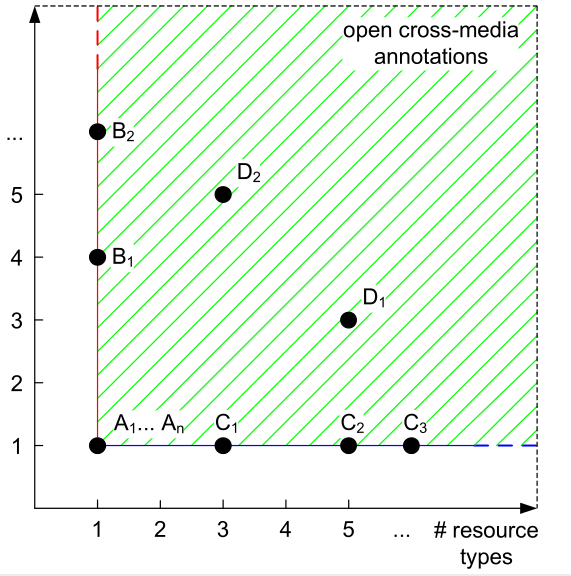
\includegraphics[scale=0.3]{filetypes.png}
		\end{column}
		\begin{column}{5cm}
			\begin{itemize}
				\item plugin based
			\end{itemize}
			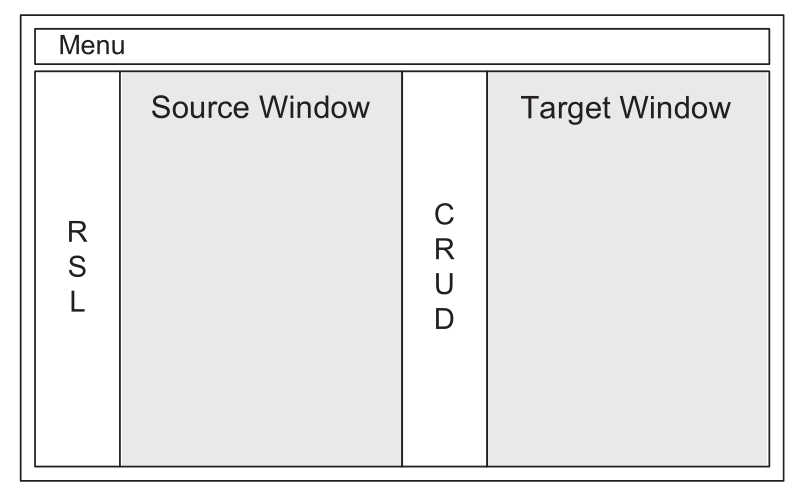
\includegraphics[scale=0.2]{layout.png}
		\end{column}
	\end{columns}
\end{frame}


\section{Contribution}
\begin{frame}
\frametitle{Contribution}
	\begin{block}{Plugin}
		\begin{itemize}
			\item Capture selection
			\item Visualise previous selections
		\end{itemize}
	\end{block}
	\begin{block}{Communication}
		\begin{itemize}
			\item Communicate with iServer through RESTfull interface
		\end{itemize}
	\end{block}
	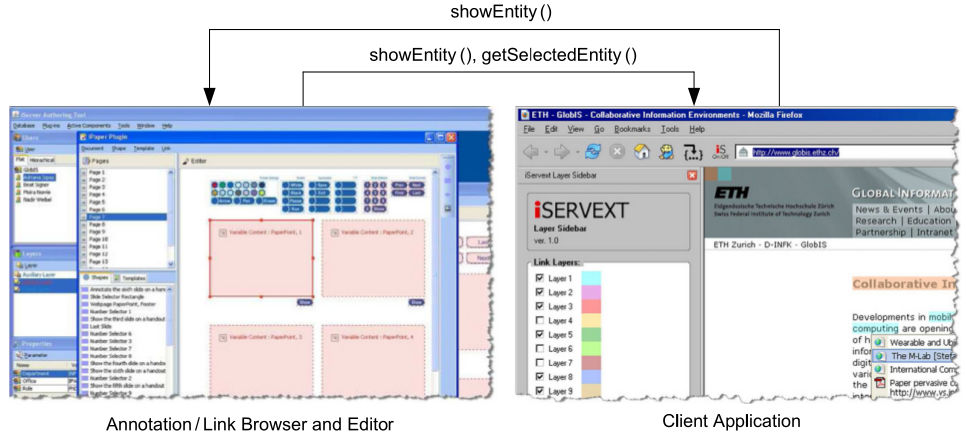
\includegraphics[scale=0.28]{client_server.png}
\end{frame}


\section{Research Question}
\begin{frame}
\frametitle{Research Question}
	\begin{block}{Problem}
		\begin{itemize}
			\item Data overload
			\item Visualisation issues
		\end{itemize}
	\end{block}
	\begin{block}{Question}
		How will we visualise all external meta data on an html-resource without cluttering the actual content
	\end{block}

\end{frame}

\begin{frame}
\frametitle{Research Question}
	\begin{block}{Problem}
		\begin{itemize}
			\item Transclusion of foreign elements
			\item Composition of components
		\end{itemize}
	\end{block}
	\begin{block}{Question}
		When deligating the visualisation of a resource to a plugin. How will it deal with translusion of foreign elements?
	\end{block}

\end{frame}


\section{Timeline}
%{
%\usebackgroundtemplate{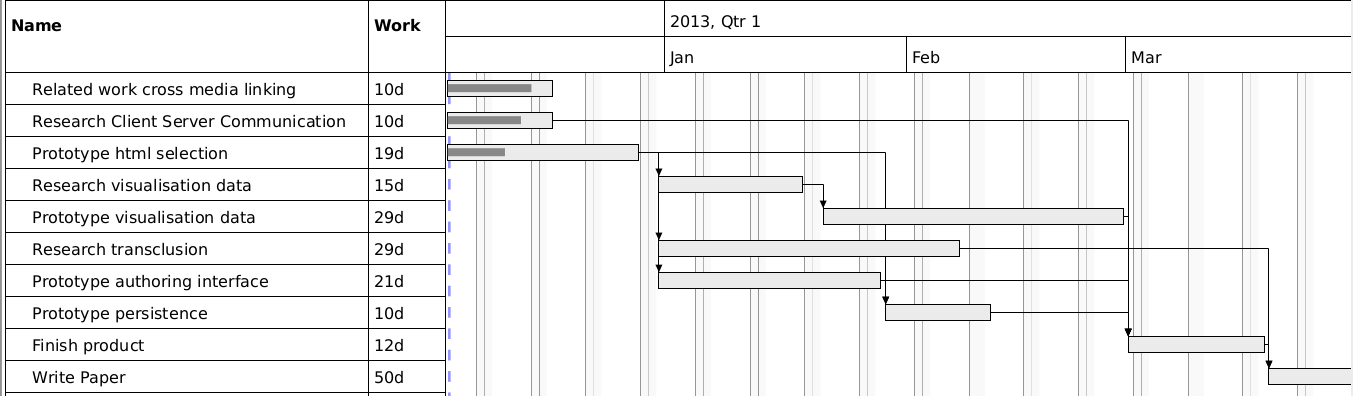
\includegraphics[keepaspectratio=false,width=1\paperwidth]{planning.png}{figure}}
%\begin{frame}[plain]
%	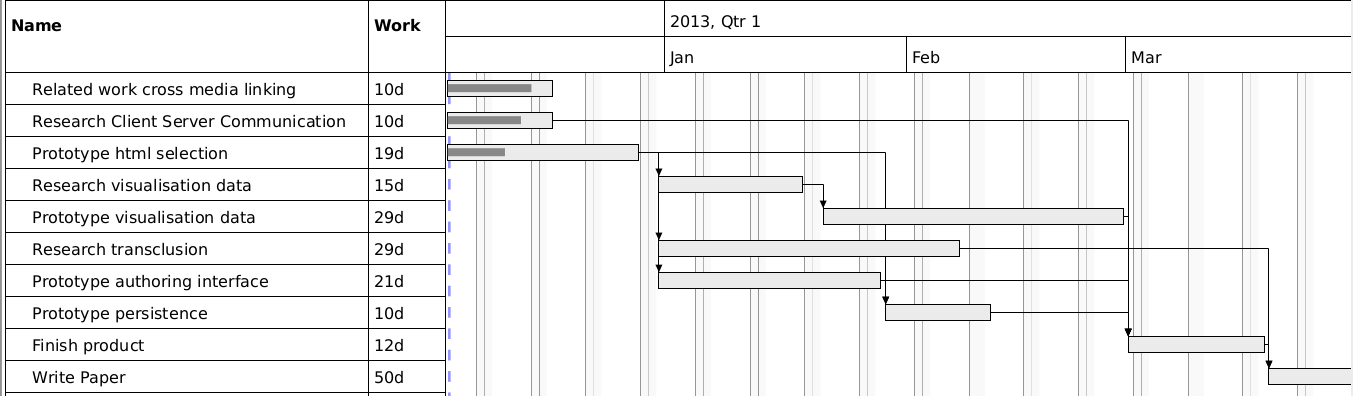
\includegraphics[width=1\paperwidth]{planning.png}
%\end{frame}
%}

\begin{frame}
\frametitle{Timeline}
	\begin{block}{What has been done}
		\begin{itemize}
			\item Related work for crossmedia linking
			\item Research client-server communication
			\item Prototype of html selection
		\end{itemize}
	\end{block}
	\begin{block}{To do}
		\begin{itemize}
			\item Research visualisation for crowd-sourced content
			\item Research transclusion issues with plugins
			\item Prototype authoring interface
			\item Prototype persistent annotations and linking
			\item Finish html visualisation prototype
			\item Finish product based on prototypes
		\end{itemize}
	\end{block}

\end{frame}
\begin{frame}
	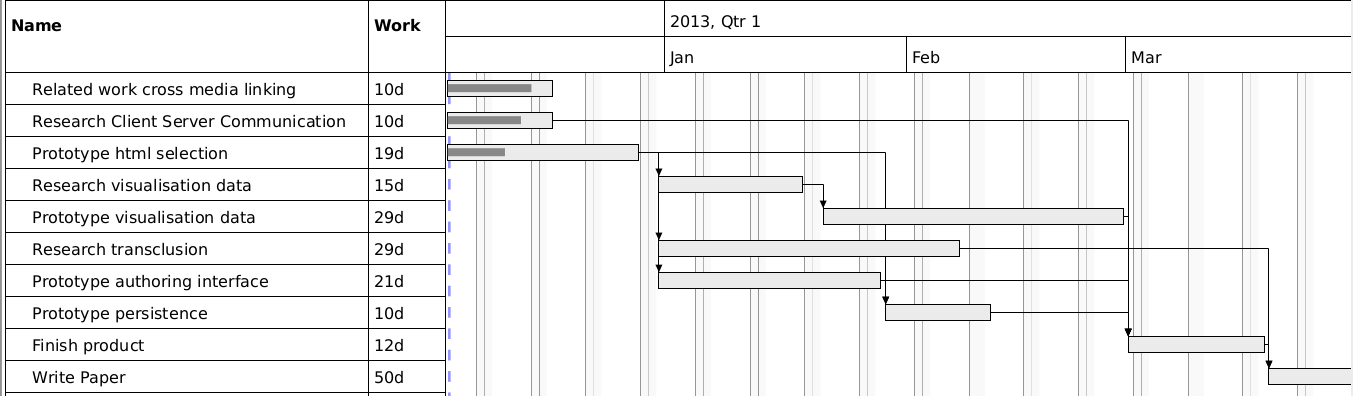
\includegraphics[width=1\paperwidth]{planning.png}
\end{frame}


\end{document}
